\documentclass{jsarticle}
\usepackage[dvipdfmx]{graphicx}
\usepackage{listings}
\begin{document}

\title{ニュートン法}
\author{中島 崇晴}
\date{提出日 2016年12月7日}
\maketitle
\begin{flushright}
    {\large 未来ロボティクス・1526084}\\
\end{flushright}

\section{目的}
ニュートン法のアルゴリズムを実装し,最低5種類の非線形方程式について解を求める。

解を求めるだけでなく,以下の要素を含める。
\begin{itemize}
    \item 解の収束の過程が分かるように途中経過を出力する。
    \item その結果をもとに,収束する様子をグラフで表されるようにする。
    \item 解が複数存在する場合もすべての解が求まるようにプログラムを拡張する。
\end{itemize}

\section{理論}
数値解析の分野において、ニュートン法またはニュートン・ラフソン法は、
方程式系を数値掲載によって解くための反復法による求根アルゴリズムの一つである。

ニュートン法では、以下の考え方に基づいて計算が行われる。

$「f(x) = 0になるような値xを探す時、ある値x1における接線の切片x2は、元の値x1より真の値xに近くなる」$

具体的にはまず、$f(x)=0$の解$\alpha$に近い値 $x_1$ を 1つとり、 関数 $y=f(x)$ のグラフ上の点  $(x_{1},f(x_1))$ における接線が、
$x$軸と交わる点の $x$ 座標 を $x_2$ とする。 このとき接線の方程式は、
\begin{equation}
    y = f'(x_1)(x-x_1)+f(x_1)
\end{equation}
となります。 ここで $y=0$ とおいて、 $x$ について解くと $x_2$ が求まる。 \\
なので、
\begin{equation}
    x_2=x_1-\frac{f(x_1)}{f'(x_1)}
\end{equation}
\\
\\
\\
\\
\\
\begin{figure}
    \centering
    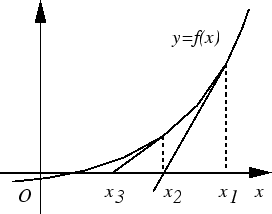
\includegraphics[bb=0 0 272 214, width=4cm]{img42.png}
    \caption{ニュートン法}
\end{figure}

次に, 点$(x_2,f(x_2))$における曲線の接線と $x$軸との交点の$x$座標を$x_3$とし, この操作を繰り返すと, 以下の数列が出てくる 
\begin{equation}
    x_1, x_2, x_3, ..., x_n, ...
\end{equation}
よって、以下の漸化式が出てくる。
\begin{equation}
    x_n+1 = x_n - \frac{f(x_n)}{f'(x_n)}
\end{equation}
式(4)を使うことにより解が出てくる。

\section{内容および方法}
まず、ニュートン法で近似する5つの非線形方程式を準備する。
\begin{eqnarray}
    x^3 + x + 1\\
    3x^3-6x^2-3x-6\\
    2sin(x)-x\\
    cos(x)-x^2\\
    e^x + x
\end{eqnarray}

式(5)を式(4)に代入し計算する工程ををコードにおろしたのが以下のである。
\begin{lstlisting}[basicstyle=\ttfamily\footnotesize, frame=single]
double formula1(double ans)
{
    return (ans-(pow(ans,3.0)+ans+1.0)/(3.0*pow(ans,2.0)+1.0));
}
\end{lstlisting}
\begin{lstlisting}[basicstyle=\ttfamily\footnotesize, frame=single]
ans = 0.0;
ans_new = formula1(ans);
while(fabs(ans-ans_new) > EPS){
    ans_new = ans;
    ans = formula1(ans_new);
}
\end{lstlisting}

更に、複数解を求めるため初期値を−10から10までの間を0.01ずつ変えていき解を出すことにした。
そのコードが以下である。
\begin{lstlisting}[basicstyle=\ttfamily\footnotesize, frame=single]
for(n=0; n<2000; n++){
    ans = -10.0 + n * 0.01;
    ans_new = formula1(ans);
    while(fabs(ans-ans_new) > EPS){
        ans_new = ans;
        ans = formula1(ans_new);
    }

    for(int i=0; i<=num_values; i++){
        if(fabs(ans-ans_old[i]) > EPS){
            discrimination = 1;
        } else {
            discrimination = 0;
            break;
        }
    }

    if(discrimination == 1){
        ans_old[num_values] = ans;
        num_values++;
        cout << ans << endl;
    }
}
\end{lstlisting}

\section{結果}
式(5)から式(9)を実際に作成したプログラムで実行した結果が以下の通りである。
\vspace{10zh}
\begin{table}[htbp]
    \begin{center}
        \begin{tabular}{c}

            \begin{minipage}{0.3\hsize}
                \begin{center}
                    \begin{tabular}{|l|c|r||r|} \hline
                        初期値 & 0\\ \hline \hline
                        1 & -1\\ \hline
                        2 & -0.75\\ \hline
                        3 & -0.686047\\ \hline
                        4 & -0.68234\\ \hline
                        5 & -0.682328\\ \hline
                        6 & -0.682328\\ \hline
                    \end{tabular}
                    \caption{式(5)}
                \end{center}
            \end{minipage}

            \begin{minipage}{0.3\hsize}
                \begin{center}
                    \begin{tabular}{|l|c|r||r|} \hline
                        初期値 & 0 & 0 & 0 \\ \hline \hline
                        1 & -3.86638  &  1 &  6.93547\\ \hline
                        2 & -2.48674  &  1 &  4.92385\\ \hline
                        3 & -1.64092  &  1 &  3.61781\\ \hline
                        4 & -1.18916  &  1 &  2.7959\\ \hline
                        5 & -1.02406  &  1 &  2.31437\\ \hline
                        6 & -1.00047  &  1 &  2.07871\\ \hline
                        7 & -1 & 1 & 2.00706\\ \hline
                        8 & -1 & 1 & 2.00007\\ \hline
                        9 & -1 & 1 & 2\\ \hline
                        10 &   -1 & 1 &  2\\ \hline
                    \end{tabular}
                    \caption{式(6)}
                \end{center}
            \end{minipage}

        \end{tabular}
    \end{center}
\end{table}

\begin{table}[htbp]
    \begin{center}
        \begin{tabular}{c}

            \begin{minipage}{0.3\hsize}
                \begin{center}
                    \begin{tabular}{|l|c|r||r|} \hline
                        初期値 & -3 & -10 \\ \hline \hline
                        1 & -2.088 & -5.8598\\ \hline
                        2 & -1.91223 &   -13.9742\\ \hline
                        3 & -1.89565 &   3.78916\\ \hline
                        4 & -1.89565 &   1.86413\\ \hline
                        5 & -1.89565 &   1.89609\\ \hline
                        6 & -1.89565 &   1.89549\\ \hline
                        7 & -1.89565 &   1.89549\\ \hline
                    \end{tabular}
                    \caption{式(7)}
                \end{center}
            \end{minipage}

            \begin{minipage}{0.3\hsize}
                \begin{center}
                    \begin{tabular}{|l|c|r||r|} \hline
                        初期値 & -10 & 5 \\ \hline \hline
                        1 &  -4.81707  &  2.26622\\ \hline
                        2 &  -2.14337  &  1.17637\\ \hline
                        3 &  -1.1417 & 0.871247\\ \hline
                        4 &  -0.863747 &  0.825308\\ \hline
                        5 &  -0.824971 &  0.824133\\ \hline
                        6 &  -0.824133 &  0.824132\\ \hline
                        7 &  -0.824132 &  0.824132\\ \hline
                        8 &  -0.824132 &  0.824132\\ \hline
                        9 &  -0.824132 &  0.824132\\ \hline
                    \end{tabular}
                    \caption{式(8)}
                \end{center}
            \end{minipage}

        \end{tabular}
    \end{center}
\end{table}

\begin{table}[htbp]
    \begin{center}
        \begin{tabular}{c}

            \begin{minipage}{0.3\hsize}
                \begin{center}
                    \begin{tabular}{|l|c|r||r|} \hline
                        初期値 & -10 \\ \hline \hline
                        1 & -0.000499377\\ \hline
                        2 & -0.500125\\ \hline
                        3 & -0.566314\\ \hline
                        4 & -0.567143\\ \hline
                        5 & -0.567143\\ \hline
                        6 & -0.567143\\ \hline
                    \end{tabular}
                    \caption{式(9)}
                \end{center}
            \end{minipage}

        \end{tabular}
    \end{center}
\end{table}

\begin{figure}[htbp]
    \begin{center}
        \begin{tabular}{c}

            \begin{minipage}{0.33\hsize}
                \begin{center}
                    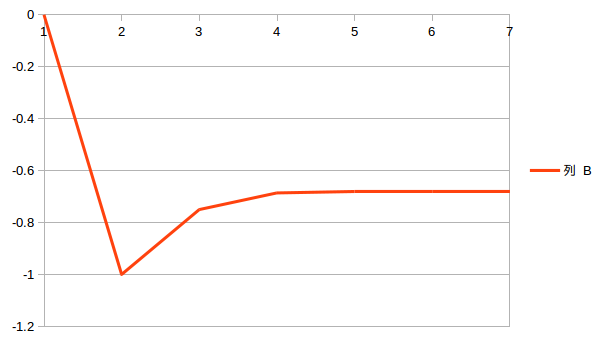
\includegraphics[bb=0 0 605 340, width=10cm]{1.png}
                    \caption{式(5)}
                \end{center}
            \end{minipage}

            \begin{minipage}{0.33\hsize}
                \begin{center}
                    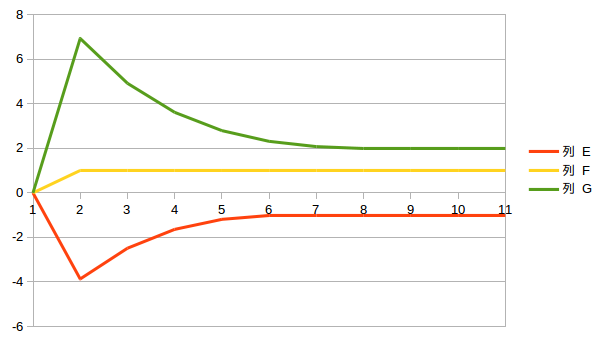
\includegraphics[bb=0 0 605 340, width=10cm]{2.png}
                    \caption{式(6)}
                \end{center}
            \end{minipage}

        \end{tabular}
        \label{fig:lena}
    \end{center}
\end{figure}

\begin{figure}[htbp]
    \begin{center}
        \begin{tabular}{c}

            \begin{minipage}{0.33\hsize}
                \begin{center}
                    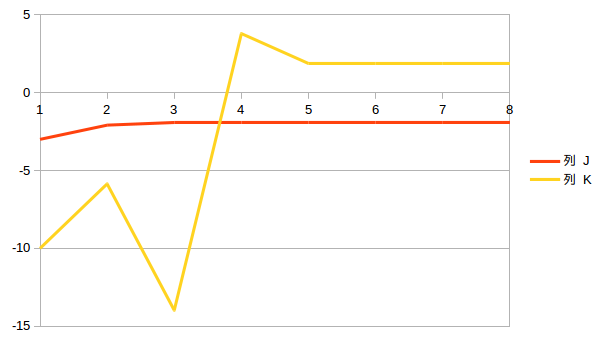
\includegraphics[bb=0 0 605 340, width=10cm]{3.png}
                    \caption{式(7)}
                \end{center}
            \end{minipage}

            \begin{minipage}{0.33\hsize}
                \begin{center}
                    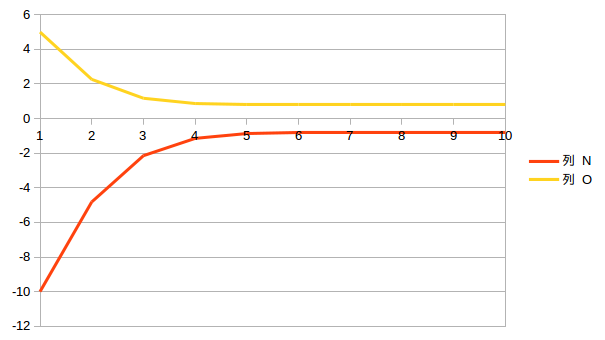
\includegraphics[bb=0 0 605 340, width=10cm]{4.png}
                    \caption{式(8)}
                \end{center}
            \end{minipage}

        \end{tabular}
        \label{fig:lena}
    \end{center}
\end{figure}

\begin{figure}[htbp]
    \begin{center}
        \begin{tabular}{c}

            \begin{minipage}{0.33\hsize}
                \begin{center}
                    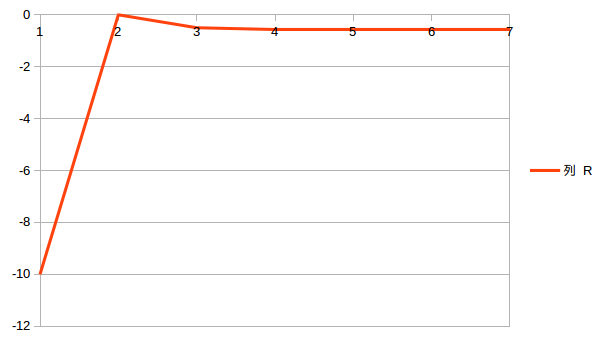
\includegraphics[bb=0 0 605 340, width=10cm]{5.png}
                    \caption{式(9)}
                \end{center}
            \end{minipage}

        \end{tabular}
        \label{fig:lena}
    \end{center}
\end{figure}

\begin{figure}
    \centering
    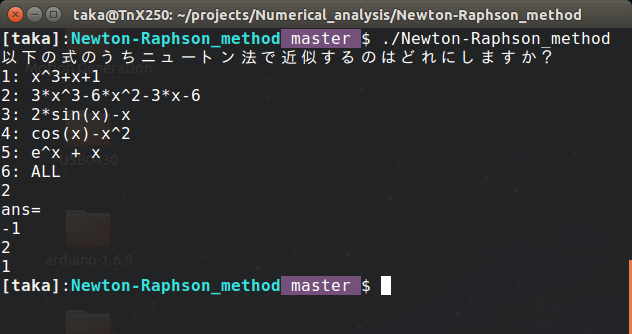
\includegraphics[bb=0 0 632 334, width=10cm]{11.png}
    \caption{式(6)を実行した場合}
\end{figure}

\section{考察}
今回、ニュートン法のアルゴリズムを実装したことによって非線形方程式の近似解を求めることが
できるので、マニュピレータの制御などが可能になった。

また、今回のレポートでLaTeXを初めて使用しました。
まだ使い方が慣れていないところがありますが、卒業論文を書くまでにはなれるようにこれからも使っていきたいと思う。

\section{付録・プログラム}
\begin{lstlisting}[basicstyle=\ttfamily\footnotesize, frame=single]
#include <iostream>
#include <cmath>

using namespace std;

#define EPS 1e-7

double formula1(double ans)
{
    return (ans-(pow(ans,3.0)+ans+1.0)/(3.0*pow(ans,2.0)+1.0));
}

double formula2(double ans)
{
    return (ans-(3*pow(ans,3.0)-6*pow(ans,2.0)-3*ans+6)/(9*pow(ans,2.0)-12*ans-3));
}

double formula3(double ans)
{
    return (ans-(2*sin(ans)-ans)/(2*cos(ans)-1));
}

double formula4(double ans)
{
    return (ans-(cos(ans)-pow(ans,2.0))/(-sin(ans)-2*ans));
}

double formula5(double ans)
{
    return (ans-(exp(ans)+ans)/(exp(ans)+1)); 
}

//double divergence(double ans){


    int main(void)
    {
        int n=0, select, num_values=0, discrimination;
        double ans, ans_new, ans_old[200];

        for(int i=0; i<200; i++) ans_old[i] = 1e-6;

        celect;

        switch(select){
            case 1:
            cout << "ans= " << endl;
            for(n=0; n<2000; n++){
                ans = -10.0 + n * 0.01;
                ans_new = formula1(ans);
                while(fabs(ans-ans_new) > EPS){
                    ans_new = ans;
                    ans = formula1(ans_new);
                }

                for(int i=0; i<=num_values; i++){
                    if(fabs(ans-ans_old[i]) > EPS){
                        discrimination = 1;
                    } else {
                        discrimination = 0;
                        break;
                    }
                }

                if(discrimination == 1){
                    ans_old[num_values] = ans;
                    num_values++;
                    cout << ans << endl;
                }
            }
            break;
            case 2:
            cout << "ans= " << endl;
            for(n=0; n<2000; n++){
                ans = -10.0 + n * 0.01;
                ans_new = formula2(ans);
                while(fabs(ans-ans_new) > EPS){
                    ans_new = ans;
                    ans = formula2(ans_new);
                }

                for(int i=0; i<=num_values; i++){
                    if(fabs(ans-ans_old[i]) > EPS){
                        discrimination = 1;
                    } else {
                        discrimination = 0;
                        break;
                    }
                }

                if(discrimination == 1){
                    ans_old[num_values] = ans;
                    num_values++;
                    cout << ans << endl;
                }
            }
            break;
            case 3:
            cout << "ans= " << endl;
            for(n=0; n<2000; n++){
                ans = -10.0 + n * 0.01;
                ans_new = formula3(ans);
                while(fabs(ans-ans_new) > EPS){
                    ans_new = ans;
                    ans = formula3(ans_new);
                }

                for(int i=0; i<=num_values; i++){
                    if(fabs(ans-ans_old[i]) > EPS){
                        discrimination = 1;
                    } else {
                        discrimination = 0;
                        break;
                    }
                }

                if(discrimination == 1){
                    ans_old[num_values] = ans;
                    num_values++;
                    cout << ans << endl;
                }
            }
            break;
            case 4:
            cout << "ans= " << endl;
            for(n=0; n<2000; n++){
                ans = -10.0 + n * 0.01;
                ans_new = formula4(ans);
                while(fabs(ans-ans_new) > EPS){
                    ans_new = ans;
                    ans = formula4(ans_new);
                }

                for(int i=0; i<=num_values; i++){
                    if(fabs(ans-ans_old[i]) > EPS){
                        discrimination = 1;
                    } else {
                        discrimination = 0;
                        break;
                    }
                }

                if(discrimination == 1){
                    ans_old[num_values] = ans;
                    num_values++;
                    cout << ans << endl;
                }
            }
            break;
            case 5:
            cout << "ans= " << endl;
            for(n=0; n<2000; n++){
                ans = -10.0 + n * 0.01;
                ans_new = formula5(ans);
                while(fabs(ans-ans_new) > EPS){
                    ans_new = ans;
                    ans = formula5(ans_new);
                }

                for(int i=0; i<=num_values; i++){
                    if(fabs(ans-ans_old[i]) > EPS){
                        discrimination = 1;
                    } else {
                        discrimination = 0;
                        break;
                    }
                }

                if(discrimination == 1){
                    ans_old[num_values] = ans;
                    num_values++;
                    cout << ans << endl;
                }
            }
            break;
            case 6:

            break;
            default:
            break;
        }
    }
    \end{lstlisting} 
    \end{document}

